\documentclass[english,11pt,openany]{article}
\usepackage{graphicx}
\usepackage{ucs}
\usepackage[utf8]{inputenc}
\usepackage[executivepaper,margin=1in]{geometry}
%\usepackage[charter]{mathdesign}
\usepackage{babel}
\usepackage{subfigure}
\usepackage{fancyhdr}
\usepackage{listings}
\usepackage{lmodern}
\usepackage{amsmath}
\usepackage{amsthm}
\theoremstyle{definition}
\newtheorem{defn}{Definition}[section]
\newtheorem{theorem}{Theorem}
\usepackage{amssymb}
\usepackage[colorlinks=true]{hyperref} 
\hypersetup{urlcolor=blue,linkcolor=black,citecolor=black,colorlinks=true}
\newtheorem{prop}{Proposition}
\usepackage[usenames,dvipsnames,svgnames,table]{xcolor}
\definecolor{light-gray}{gray}{0.70}

\begin{document}
\begin{titlepage}

\title{
\hspace{0.75cm}Backward Stochastic Differential Equation 
\newline
\hspace{0.35cm}\textbf{Derivative Method : Analysis}
}

\author{Majdi Rabia}
\date{
\hspace{2.5cm} 
\newline
}

\maketitle

\section{Introduction}

%\hspace{1cm} \includegraphics[width=10cm]{}

Simulations on American Options Pricing in high dimensions work well as they do not involve a noisy process in regression step. This is the case in our bid-ask problem, following the BSDE: 

\begin{equation}
-dY_t=f(t,Y_t,Z_t)dt - Z_tdW_t  
\end{equation}

where 

\[
\left\{
\begin{aligned}
f(t,Y_t,Z_t) & =  - \theta Z_t - rY + (R-r)(Y-\frac{Z_t}{\sigma})^-\\
Z_t & = \sigma \sum_{i = 1}^{p} \Phi^i_t\\
\theta &= \frac{\mu - r}{\sigma}
\end{aligned}
\right.
\]

Let's compare our results to Gobet's simulation with the following parameter : 

\begin{tabular}{c|c|c|c|c|c|c|c|c|c|c}
	$T$ & $S_0$  & $K$ & r & R & $\mu$ & $\sigma$ \\
	\hline
	0.5  & 100  & 100  & $0.04$ & $0.06 $ & $0.06$ & 0.2
\end{tabular}

%\begin{figure}[!htb]
%	\centering
%	\includegraphics[width=10cm]{.png} 
%\end{figure}
\newpage

\section{Regression}

\begin{displaymath}
Z_{t_i} = \frac{1}{\Delta t_i}\mathbb{E}[Y_{t_{i + 1}} \Delta B_{t_i}  | \mathcal{F}_{t_i}]
\end{displaymath}

\begin{displaymath}
Y_{t_i} = \mathbb{E}[Y_{t_{i + 1}} | \mathcal{F}_{t_i}] +  f(t_i,S_{t_i}, Y_{t_{i + 1}}, Z_{t_i})\Delta t_i
\end{displaymath}

\section{Derivative Iteration}

This method uses the fact $Z_t = \sigma S_t \frac{\partial w}{\partial S}$ where $Y_t = w(t, S_t)$

\begin{itemize}
	\item $\forall t_i$ we compute once the regression using for example a RandomForest (in high dimensions), or a least square estimator on polynomial basis (one dimension). 
	
	\item Assumption : $Y_{t_i} = \hat{f}(S_{t_i})$
	
	Gaussian approximation : $\hat{f}(x) = \sum_{i=1}^{N} \frac{\omega(x, x_i)}{\sum_{j=1}^{N}\omega(x, x_j)}Y_i$ where i denotes the i'th simulation
	
	where the weight $\omega(x, x_i) = e^{- \frac{(x - x_i)^2}{2l^2}}$
	
	l being a parameter depending on the scale of the given data (the smaller, the better)
	
	\item Once $\hat{f}$ is computed, as it was chosen derivable on purpose, we compute the derivative $\hat{f}'$
	
	\item We set $Z_{t_i} = \sigma S_{t_i} \hat{f}'(S_{t_i})$
\end{itemize}

We iterate this method at every step, to get the smoother $Z$ possible. 

\section{Simulations}

\subsection{1st : Price convergence}
\begin{tabular}{c|c|c|c|c|c|c|c|c|c|c}
	N\_particles & m\_discretization  & N\_run & n\_picard & nearest\_neighbors & l \\
	\hline
	1000  & 12  & 20  & 3 & 100 & 1.0
\end{tabular}

\vspace{1cm}

\textbf{Theoretical Price : 7.15}


\begin{table}[]
		\centering
		\caption{Simulation}
		\vspace{1cm}
		\begin{tabular}{lll}
			Run Number & Time in seconds &  Price \\
			\hline
			run 1	&	3.591 &	7.428653384 \\
			run 2	&	4.751&	7.042321827\\
			run 3	&	3.932&	7.257010564\\
			run 4	&	3.618&	6.917118799\\
			run 5	&	3.223&	7.171610637\\
			run 6	&	4.307&	7.090800489\\
			run 7	&	3.75&	7.206036474\\
			run 8	&	3.97&	6.952620543\\
			run 9	&	3.494&	7.648404958\\
			run 10	&	4.907&	6.741787516\\
			run 11	&	4.204&	7.696553542\\
			run 12	&	4.136&	6.818502178\\
			run 13	&	4.403&	7.775232407\\
			run 14	&	4.081&	6.780866829\\
			run 15	&	4.013&	7.180213783\\
			run 16	&	3.572&	7.485186614\\
			run 17	&	4.204&	7.258745764\\
			run 18&		4.473&	7.270984402\\
			run 19	&	3.673&	6.800149302\\
			run 20	&	3.942&	7.035487849\\
		
		\end{tabular}
		
		\begin{tabular}{lllll}
			mean & std & 95\% confidence interval & min & max \\
			\hline
			  7.1779 	&	0.3088 & [7.1476, 7.2082] &	6.7418&	7.7752
		\end{tabular}
\end{table}
\newpage
\newpage


\paragraph{Remark}

Even with a smoother Z, we can notice a high variance. Of course, the number of $1000$ particles being limited, it might be a cause. I am working on getting the same result with a bigger N\_particles


\subsubsection{Analysis of the number of neighbors on the Price}

\begin{figure}[!htb]
	\centering
	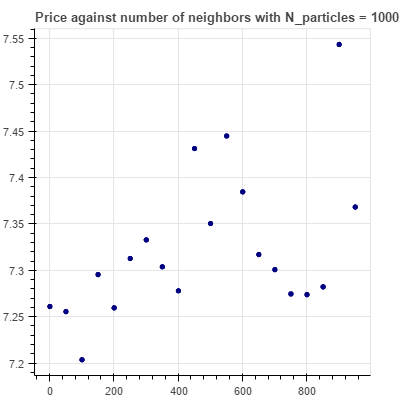
\includegraphics[width=8cm]{y_against_nn_mrun.png} 
\end{figure}


\paragraph{Remarks}

Given the variance of one run with n\_neighbors, this simulation has been made with several runs (5) for each point ... 
The results are not the one we would have expected, as a number of neighbours increasing seem to be less precise. 
My assumption is that given the small difference between $r$ and $R$ ($0.06 - 0.04$), $Z_t$ might not be so important in this computation.  

\subsection{Analysis of the parameter l}

\begin{figure}[!htb]
	\centering
	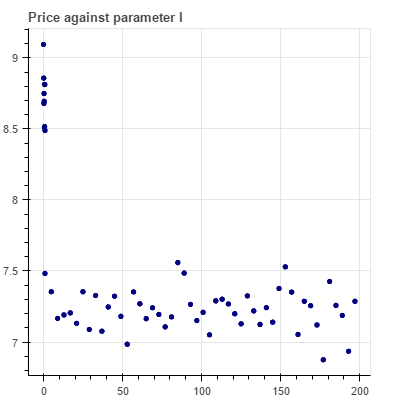
\includegraphics[width=8cm]{y_against_l_mrun.png} 
\end{figure}

\newpage

\paragraph{Remarks}

As before, given the variance of one run , this simulation has been made wwith 5 runs for each point. 
A value near 0 for l parameter gives for every point $i$ (at each step $t$) a very small weight. That explains the values we have around 0. 

We should observe for big values of l a bigger error (as for l near 0), but we do not. Indeed, when l is bigger than $(x - x_i)$, the weight $\omega$ should be almost equal to 1! Giving then the same weight for each point $Y_i$ and we would have a simple Monte-Carlo. 

My assumption is that we get $\mathbb{E}[Y_{t_i}] \forall t_i$ instead of $Y_{t_i}$, which does not seem to be much different, and would explain why bigger l do not give worse values.

\subsection{Plotting the noisy Process Z against the Stock Price X}

\begin{figure}
	
	\subfigure[Figure A]{\label{fig:a}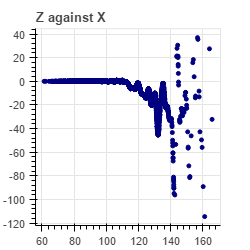
\includegraphics[width=40mm]{t=11.png}}
	\subfigure[Figure B]{\label{fig:b}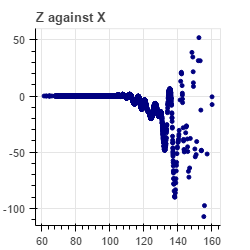
\includegraphics[width=40mm]{t=10.png}}
	\subfigure[Figure C]{\label{fig:c}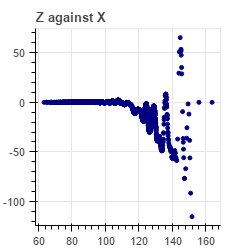
\includegraphics[width=40mm]{t=9.png}}
	\subfigure[Figure D]{\label{fig:d}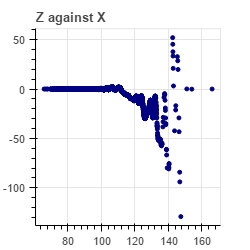
\includegraphics[width=40mm]{t=8.png}}
	\subfigure[Figure E]{\label{fig:e}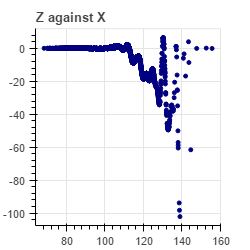
\includegraphics[width=40mm]{t=7.png}}
	\subfigure[Figure F]{\label{fig:f}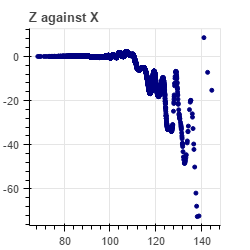
\includegraphics[width=40mm]{t=6.png}}
	\subfigure[Figure G]{\label{fig:g}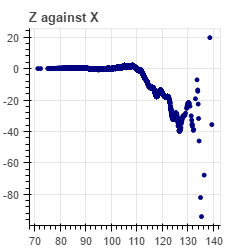
\includegraphics[width=40mm]{t=5.png}}
	\subfigure[Figure H]{\label{fig:h}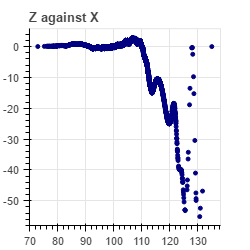
\includegraphics[width=40mm]{t=4.png}}
	\subfigure[Figure I]{\label{fig:i}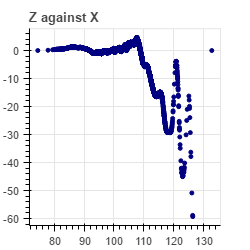
\includegraphics[width=40mm]{t=3.png}}
	\subfigure[Figure J]{\label{fig:j}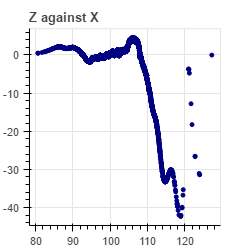
\includegraphics[width=40mm]{t=2.png}}
	\subfigure[Figure K]{\label{fig:k}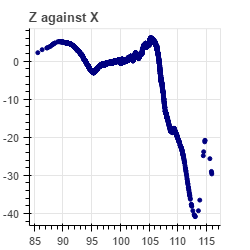
\includegraphics[width=40mm]{t=1.png}}
	\caption{Z against X for a 12 steps discretization}
	\label{fig:test}
\end{figure}

\newpage

\subsection{Time analysis}

\begin{figure}[!htb]
	\centering
	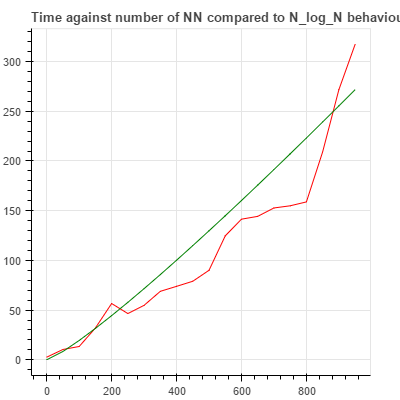
\includegraphics[width=8cm]{time_analysis.png} 
\end{figure}


\paragraph{Remark}

I plotted here an $Nlog(N)$ behaviour against a number of neighbours increasing, along with the time taken for each number of NN. 
We can notice how the two functions seem to behave samely here . 

\end{titlepage}
\end{document}]